\documentclass[mathserif,final,hyperref={pdfpagelabels=false}]{beamer} %

\usepackage[english]{babel}
%\usepackage[latin1]{inputenc}
\usepackage[ansinew]{inputenc}
\usepackage{amsmath,amsthm, amssymb,latexsym}
\usepackage{graphicx}
\usepackage{setspace}
\usepackage{subfigure}

\usepackage[T1]{fontenc}
%\renewcommand{\sfdefault}{lhv}
%\usepackage[euler-hat-accent]{eulervm}

\usepackage[small,vertical,titleright]{posterlti}


% ---------- Definitionen ----------
\def\d{ \mathrm{d} }											% integral d
\def\I{ \mathrm{i} }											% imaginary unit
\def\E{ \mathrm{e} }											% e
\def\uC{ \mathbb{T} }											% unit circle
\def\uD{ \mathbb{D} }											% unit disk

\def\H{ \mathcal{H} }											% Hilbert space

\def\RN{ \mathbb{R} }											% real numbers
\def\CN{ \mathbb{C} }											% complex numbers
\def\ZN{ \mathbb{Z} }											% integers
\def\NN{ \mathbb{N} }											% non-negative integers

\def\bss{ \boldsymbol{s} }								% Sequence s
\def\bssigma{ \boldsymbol{\sigma} }				% Sequence sigma

\def\Tr{ \mathrm{S} }											% translation operator
\def\Pr{ \mathrm{P} }											% projection
\def\Nu{ V }

\DeclareMathOperator*{\cls}{\overline{span}}			% closed linear span
\DeclareMathOperator*{\argmin}{arg\, min}					% argmin
\DeclareMathOperator*{\argmax}{arg\, max}

\input math.tex

% ----------------------------------




\title{\huge Image segmentation with superpixel MRF and shape priors}
\author{\bfseries Fanny Yang}
\institute{Department for Electrical Engineering and Computer Science, UC Berkeley}
\date{May 13$^{th}$, 2014}
\setfootlinelti{CS281A - Class Project Poster Session}{Fanny Yang}


\begin{document}
\begin{frame}
\begin{columns} 
%%%%%%%%%%%%%%%%%%%%%%%%%%%%%%%%%%%%%%%%%%%%%%%%%%%%%%%%%%%%%%%%%%%%%%%%%% 
%%%%%%%%%%%%%%%%%%%%%%%%%%%%%%%%%%%%%%%%%%%%%%%%%%%%%%%%%%%%%%%%%%%%%%%%%% 
% COLUMN 1
%%%%%%%%%%%%%%%%%%%%%%%%%%%%%%%%%%%%%%%%%%%%%%%%%%%%%%%%%%%%%%%%%%%%%%%%%% 
%%%%%%%%%%%%%%%%%%%%%%%%%%%%%%%%%%%%%%%%%%%%%%%%%%%%%%%%%%%%%%%%%%%%%%%%%%
\begin{column1lti}


% ============================== Motivation ==============================
\begin{blocklti}{Motivation -- Gene expression analysis}

\begin{itemize}
\item Different embryos are used for each gene and stage
\item Need a map to a standard template for comparability
\item[$\Rightarrow$] One method: image segmentation
\item Challenge 1: Low intensity contrasts, hard to segment even for humans
\item Challenge 2: Need detailed information from very high resolution image
\item Known: Shape and positions roughly follow a given template
\item[$\Rightarrow$] Approach: Combining superpixels and shape priors using an MRF
\end{itemize}

\begin{figure}[htbp]
\centering
\subfigure{
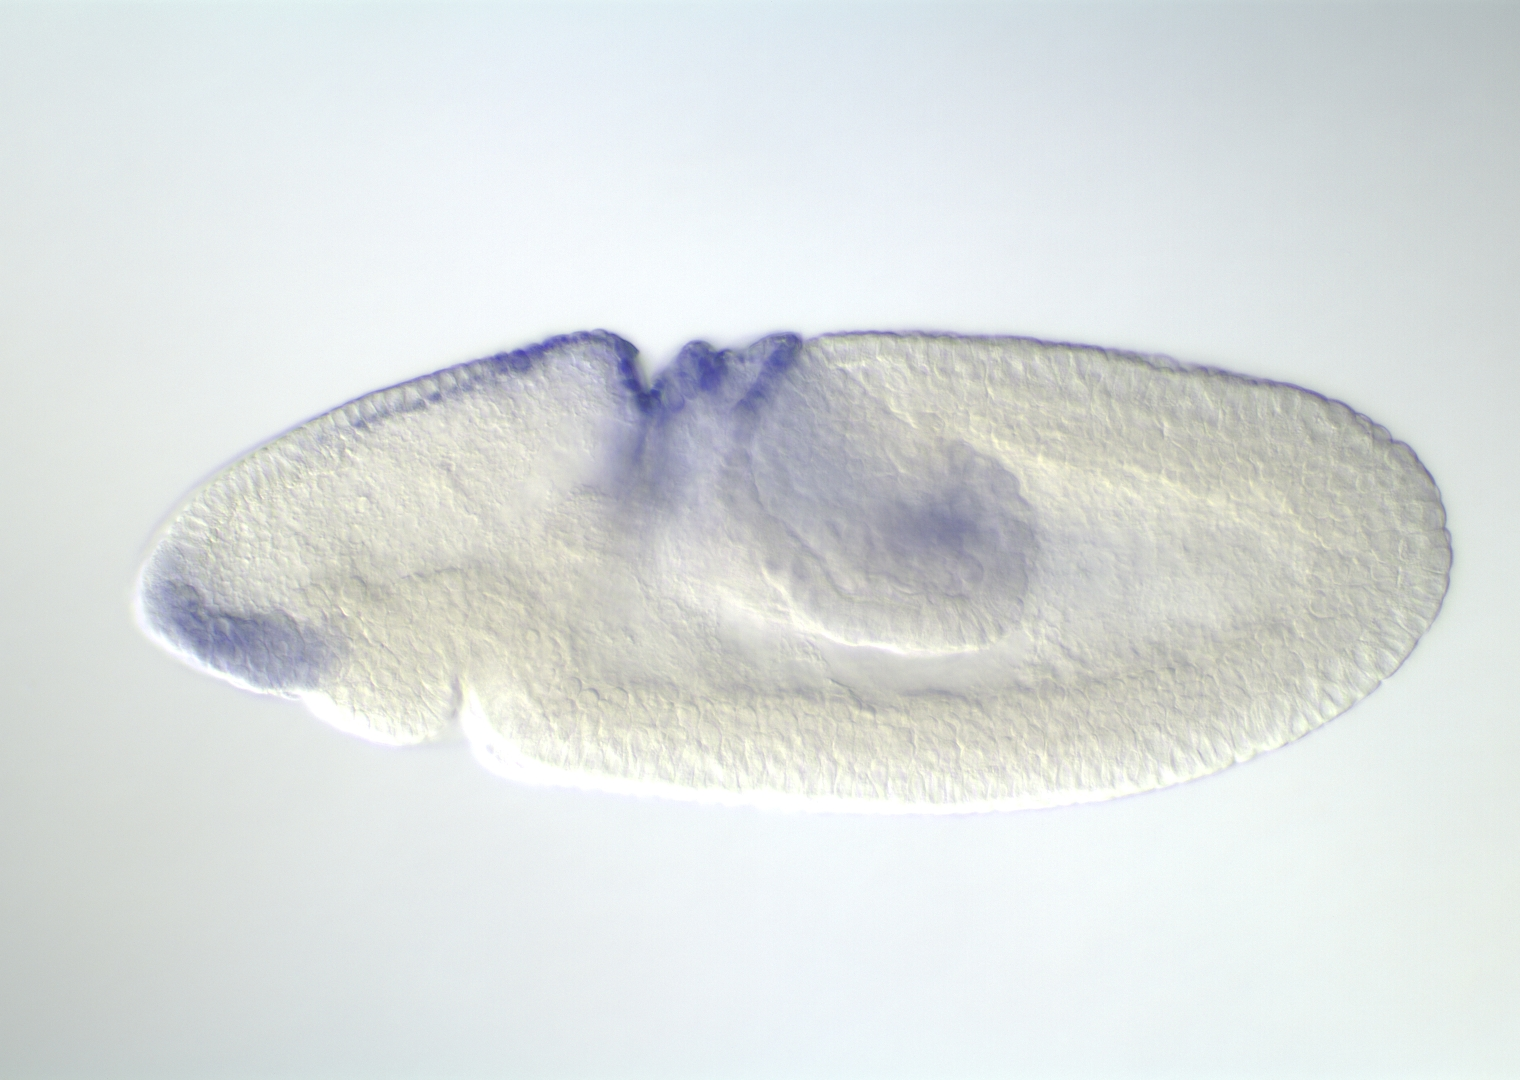
\includegraphics[width=160mm]{insitu51843.jpg}
}
\subfigure{
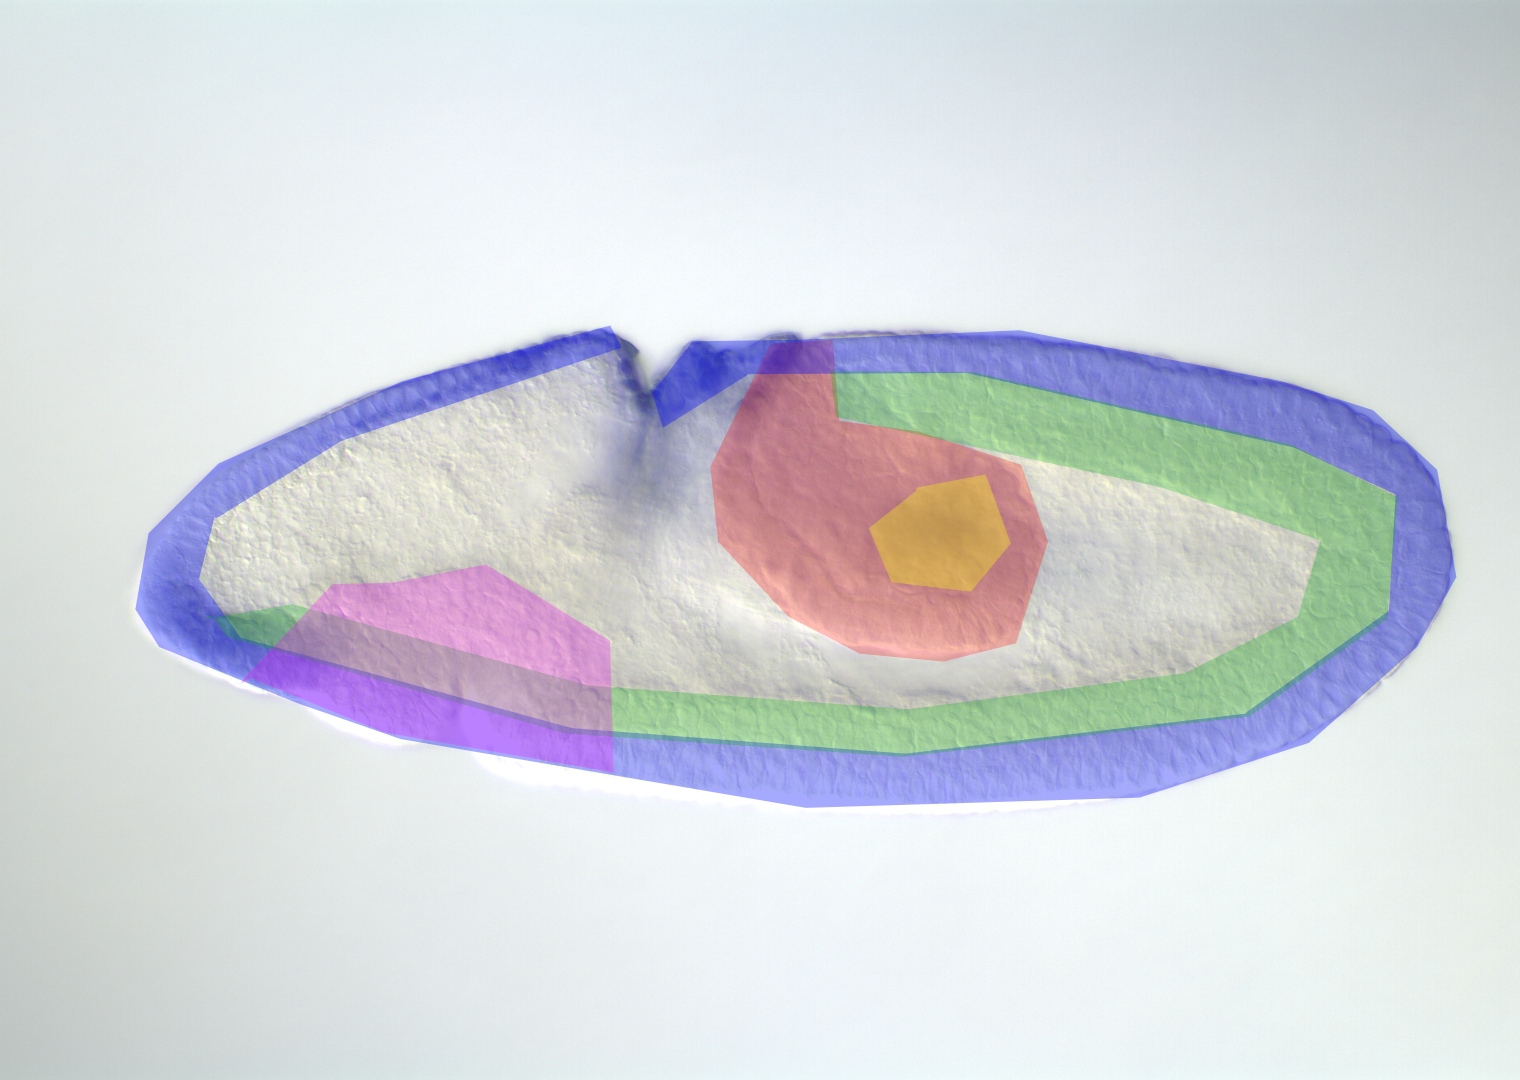
\includegraphics[width=160mm]{segmentedFruitfly.png}
}
\end{figure}
\end{blocklti}
% ========================================================================

\vfill


% ============================== MRF model ==============================
\begin{blocklti}{Image segmentation with shape priors}


\structure{\bfseries Image segmentation }

\begin{itemize}
\item Given pixel features $x$, obtain labels $y$, pixel coordinates $i$ 
\item Minimization of energy, equivalent with maximization of the likelihood
\begin{equation*}
y = \argmin_y E(y,x) \iff y = \argmax_y p(y|x) 
\end{equation*}
with $p(y|x) \propto \exp(-E(y,x))$
\item Discriminative models (CRF) vs. generative models (MRF) for $p(y|x)$.
\item Incorporate priors via generative models $p(y|x) \propto p(x,y)$.
\end{itemize}

\vspace{1ex}

\structure{\bfseries Incorporating shape priors using level set functions}
\begin{itemize}
\item Model contour of the set $S= \{i\in \Nu: y_i =1\}$  as the zero level set of a function $\phi(i)$, so $S = \{i\in\Nu: \phi(i) = 0\}$
\item Use as additional random variable to obtain $p(y,\phi|x) \propto p(x,y|\phi)p(\phi)$
\item Make $p(\phi)$ dependent on prior information
\begin{equation*}
p(\phi|\tilde{\phi}) = \exp(-( E_{int}(\phi) + E_{prior}(\phi,\tilde{\phi})))
\end{equation*}
with $E_{int}$ e.g. penalizing length of the contour and a nonparametric kernel density estimate for 
\begin{align*}
\exp(- E_{prior}(\phi,\tilde{\phi})) = \sum_{i=1}^N \exp\left(-\frac{1}{2\sigma^2}d^2(H_\epsilon(\phi),H_\epsilon(\phi_i))\right)
\end{align*}
where $d$ is similar to the Hamming distance between two functions
\item Minimization using update equation
\begin{equation*}
\frac{\partial \phi}{\partial t} = -\frac{\partial E_{int}(\phi)}{\partial \phi} - \frac{\partial E_{prior}(\phi)}{\partial \phi}  \label{labelset_update}
\end{equation*}
\end{itemize}

\hrule

\vspace{2ex}

\begin{thebibliography}{1}
\begin{spacing}{2.0}
\bibitem{Cremers}
{ \footnotesize Cremers, Daniel, Stanley J. Osher, and Stefano Soatto. ``{Kernel density estimation and intrinsic alignment for shape priors in level set segmentation}'' \emph{ International Journal of Computer Vision} 69.3 (2006): 335-351.} 

%% M.~Unser and A.~Aldroubi, ``{A General Sampling Theory for Nonideal Acquisition
%%   Devices},'' \emph{{IEEE} Trans. Signal Process.}, vol.~42, no.~11, pp.
%%   2915--2925, Nov. 1994.}

 \vspace{1ex}

\bibitem{ChanVese}
{ \footnotesize Chan, Tony F., and Luminita A. Vese. ``{Active contours without edges.}'' \emph{ Image processing, IEEE} transactions on 10.2 (2001): 266-277..}
%% \bibitem{MPE_IEEE_SP_11}
%% { \footnotesize T.~Michaeli, V.~Pohl, and Y.~C. Eldar, ``{U-Invariant Sampling: Extrapolation
%%   and Causal Interpolation from Generalized Samples},'' \emph{{IEEE} Trans.
%%   Signal Process.}, vol.~59, no.~5, pp. 2085--2100, May 2011. }
\end{spacing}
\end{thebibliography}


\end{blocklti}
% =======================================================================

\vfill

% ============================== Own model  ==============================

\begin{blocklti}{Combining superpixel MRF and shape priors}

\structure{\bfseries Variables}
\begin{itemize}
\item Graph: $G(V, E)$ with $V$ set of nodes, $E$ set of edges
\item Observed superpixel features (intensity, texture): $x_i \in \RN^d$, $i\in V$
\item Latent variables: Labels $y_i \in {0,\dots,k}, i\in V$, level set function $\phi$
\item Training data: Segmented shapes $\tilde{\phi}$
\item Joint probability distribution:
\begin{align*}
p(x,y,\phi) &=  \prod_{i\in \Nu} \psi(x_i,y_i)  \prod_{(i,j)\in E} \psi(y_i,y_j)\prod_{i\in \Nu} p(y_i|\phi)p(\phi) \label{total_joint}\\
&=: \prod_{i\in \Nu} p(x_i|y_i)\prod_{(i,j)\in E} p(y_i,y_j) \prod_{i\in \Nu} p(y_i|\phi)p(\phi|\tilde{\phi})\nonumber
\end{align*}
\end{itemize}

\begin{columns}[t]

\begin{column}{0.5\linewidth}
%\centering
\structure{\bfseries Probability model}

\begin{itemize}
\item Gaussian mixture for the conditional probability
\beqs
p(x_i|y_i = k) = \N(\mu_k,\Sigma_k)
\eeqs
\item Pairwise (edge) potentials %Penalty for differently labeled neighbors
\beqs
p(y_i,y_j) \propto \theta_1 \Indi_{y_i\neq y_j} + \theta_2 \Indi_{y_i=y_j}
\eeqs
\item Conditional probability of $y$ given $\phi$
\beqs
p(y_i|\phi) = \left(\frac{1}{1 + \E^{-\lambda \phi(i)}}\right)^{y_i} \left(\frac{1}{1 + \E^{\lambda \phi(i)}}\right)^{1-y_i}
\eeqs
\end{itemize}

\end{column}

\begin{column}{0.5\linewidth}

  \vspace{-2ex}
  \begin{figure}[t]
  \centering
  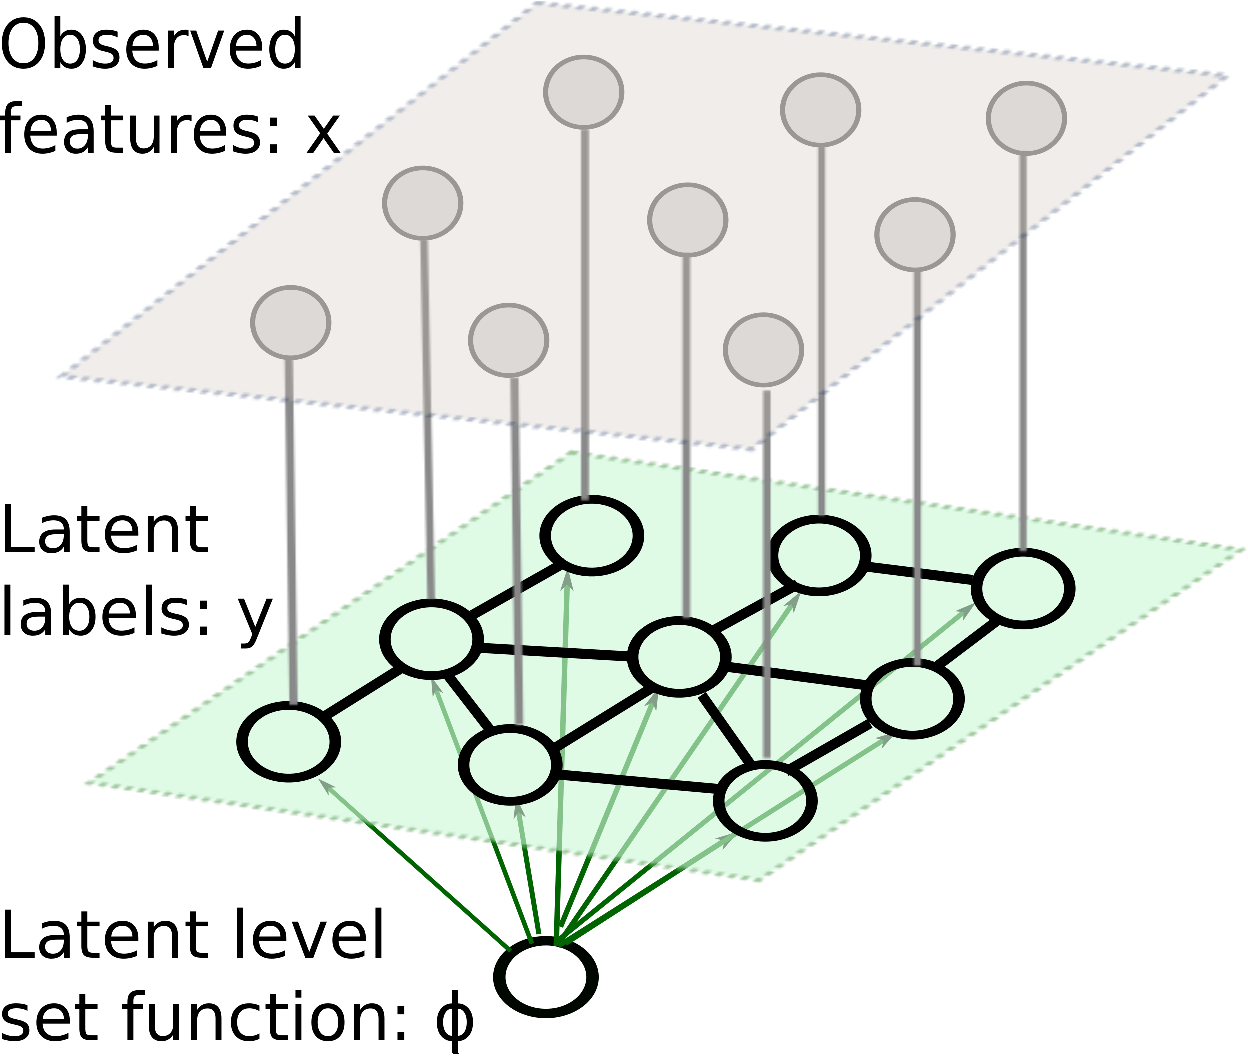
\includegraphics[width=160mm]{MRF.pdf}
  \end{figure}

 %% \begin{column}{0.45\linewidth}

 %% \end{column}

\end{column}

\end{columns}

\end{blocklti}
% =======================================================================================

%\vfill

%% % ============================== PROBLEM =============================================
%% \begin{colorblocklti}[yellow!90!white]
%% \begin{center}
%% {\bfseries Maximizing $p(x,y,\phi)$ is computationally intractable!}
%% \end{center}

%% \end{colorblocklti}
%% % ====================================================================================

%% \vfill


%

\end{column1lti}



%%%%%%%%%%%%%%%%%%%%%%%%%%%%%%%%%%%%%%%%%%%%%%%%%%%%%%%%%%%%%%%%%%%%%%%%%% 
%%%%%%%%%%%%%%%%%%%%%%%%%%%%%%%%%%%%%%%%%%%%%%%%%%%%%%%%%%%%%%%%%%%%%%%%%%
% column 2
%%%%%%%%%%%%%%%%%%%%%%%%%%%%%%%%%%%%%%%%%%%%%%%%%%%%%%%%%%%%%%%%%%%%%%%%%%
%%%%%%%%%%%%%%%%%%%%%%%%%%%%%%%%%%%%%%%%%%%%%%%%%%%%%%%%%%%%%%%%%%%%%%%%%%
\begin{column2lti}


% ============================== PROBLEM =============================================
\begin{colorblocklti}[yellow!90!white]
\begin{center}
{\bfseries 
Exact inference for $p(y,\phi|x)$ is not computationally tractable $\Rightarrow$ Variational inference}
\end{center}

\end{colorblocklti}
% ====================================================================================

\vfill

% ============================== Main Result ==============================
\begin{blockredlti}{Segmentation Algorithm}

\structure{\bfseries Structured variational inference}
\begin{itemize}
\item Approximate $p(y,\phi|x)$ by an easier probability distribution
\beqs
Q(y,\phi|x,a,b,\tilde{\phi}) = Q_M(y|x,a)Q_D(\phi|b,\tilde{\phi}) 
\eeqs with
$Q_M(y|x,a) \propto \prod_{i\in \Nu} p(x_i|y_i)p(y_i|a_i)$ and $Q_D(\phi|b) \propto  \prod_{i\in\Nu} p(b_i|\phi)p(\phi|\tilde{\phi})$
\item Minimize the Kullback Leibler distance $KL(Q||P)$ which yields the fixed point equation
\begin{align*}
\log p(y_i|a_i) &= \EE_{Q_D} \log p(y_i|\phi) \\
\log p(b_i|\phi) &= \EE_{Q^i_M} \log p(y_i|\phi)  
\end{align*}
\item This yields $-E(\phi) = \log Q_D(\phi|b) \propto  \log p(\phi|\tilde{\phi}) + \EE_{Q_M^i}\log p(y_i|\phi)$ and thus the update equation for finding $\phi^* = \argmax Q_D(\phi|b)$. 
\begin{equation}
\label{combined_update}
\frac{\partial \phi}{\partial t} = -\frac{\partial E_{int}(\phi)}{\partial \phi} - \frac{\partial E_{prior}(\phi)}{\partial \phi}  -  \EE_{Q_M^i}\frac{\partial}{\partial \phi}\log p(y_i|\phi)
\end{equation}
\item Then choose $y = \argmax_y Q_M(y|x,a)$.
\end{itemize}



\structure{\bfseries Algorithm}

\begin{itemize}
\item Initialize $p(y_i|a_i)$ by a uniform distribution.
\item Step $k$.
\begin{enumerate}
\item In order to calculate $Q_M(y_i|x_i,a)$ estimate the parameters of $p(x_i|y_i)$ (which are $\mu_k,\Sigma_k$) using the EM algorithm %latent variable $y_i$ and the EM algorithm
\item Given approximate $Q_M(y_i|x_i,a)$ using loopy belief propagation/mean field inference.
\item Calculate $\log p(b_i|\phi) = \EE_{Q_M^i} \log p(y_i|\phi)$.
\item Calculate $\phi^* = \argmax_{\phi} Q_D(\phi|b)$ using \eqref{combined_update}
\item Approximate $p(y_i|a_i) = \exp(\EE_{Q'_D} \log p(y_i|a_i))= p(y_i|\phi^*)$.
\end{enumerate} 
\item Upon termination: $y_i = \max_k Q_M(y_i = k|x,a)$. 
\end{itemize}

\end{blockredlti}

\vfill


% ======================================== EXAMPLE - CAUSAL SPLINE INTERPOLATION ========================================
\begin{examplelti}[Example -- Touching embryos]

\structure{\bfseries Problem}

Separate the embryo of interest in the ``middle'' using shape prior.

\structure{\bfseries Segmentation results}
%Results of the superpixel algorithm. 
 \begin{figure}[htbp]
  \centering
  \subfigure{
  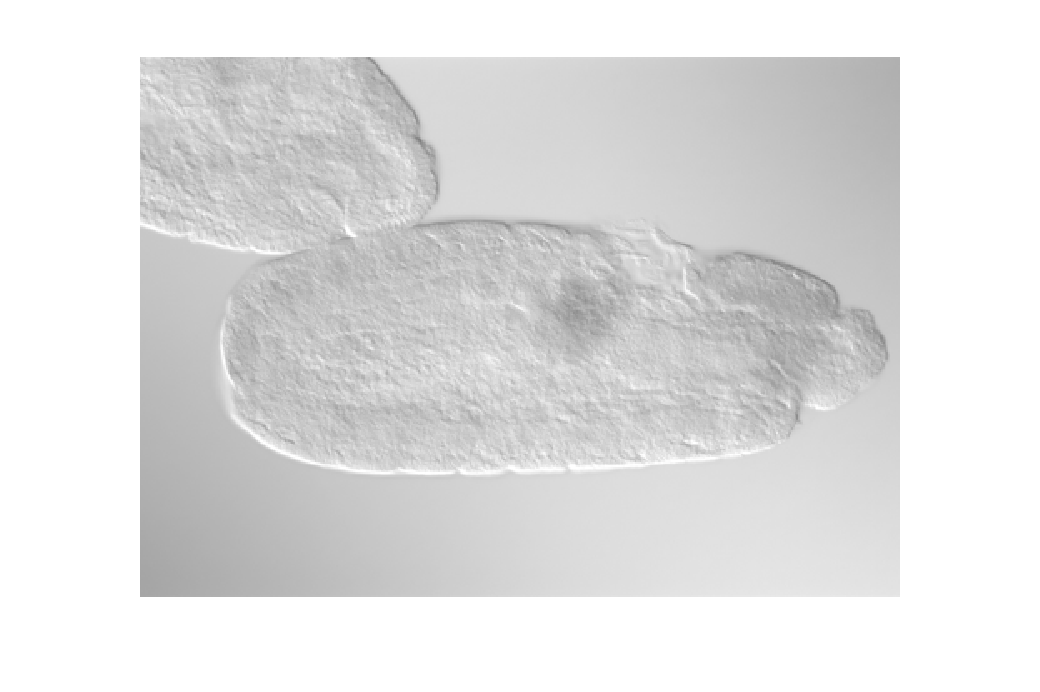
\includegraphics[width=150mm]{touching2.pdf}
  }
  \subfigure{
  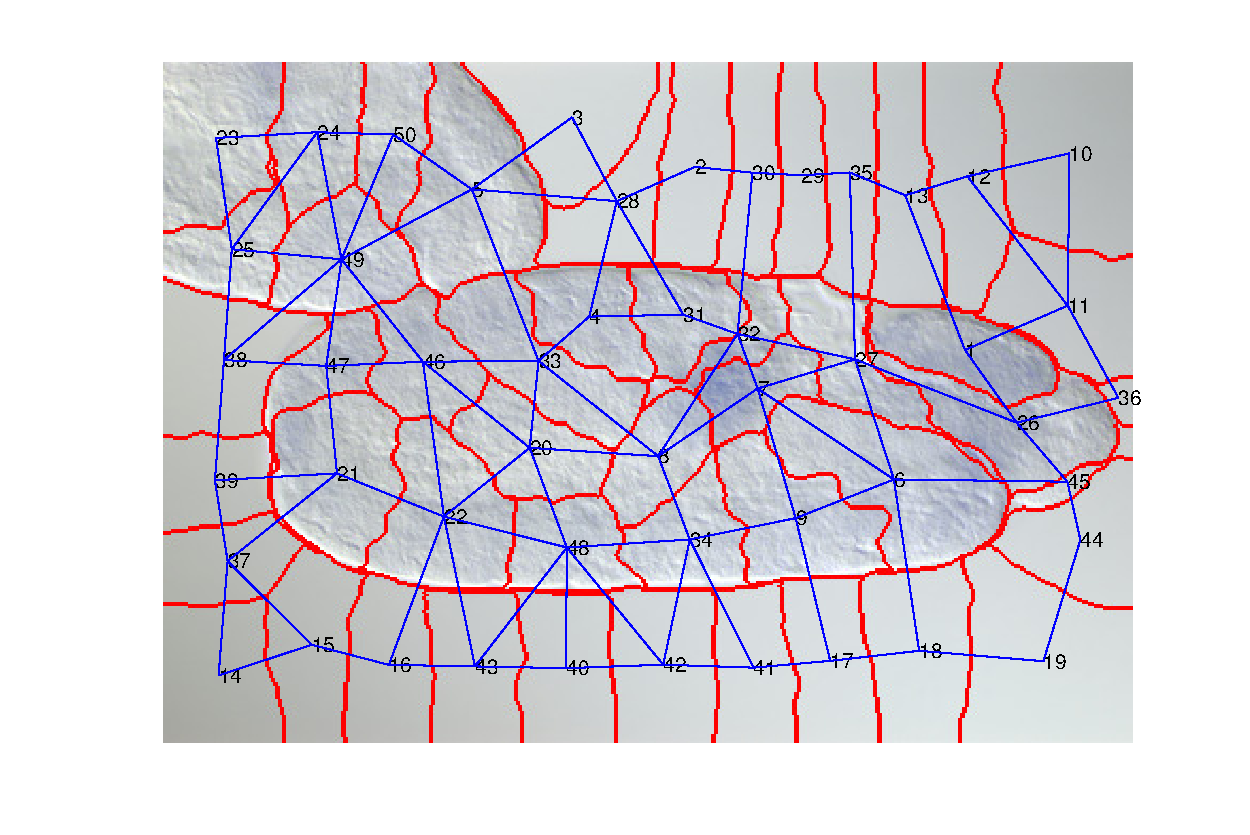
\includegraphics[width=150mm]{fruitflyEmbSuperPixelEg.pdf}
 }  
\caption{Left: Original picture. Right: Superpixel segmentation with edge structure for MRF (on a resized image)}
\label{Superpixels}
 \end{figure}

%Segmentation results running MRF and level set segmentation on superpixel
 \begin{figure}[htbp]
  \centering
  \subfigure{
  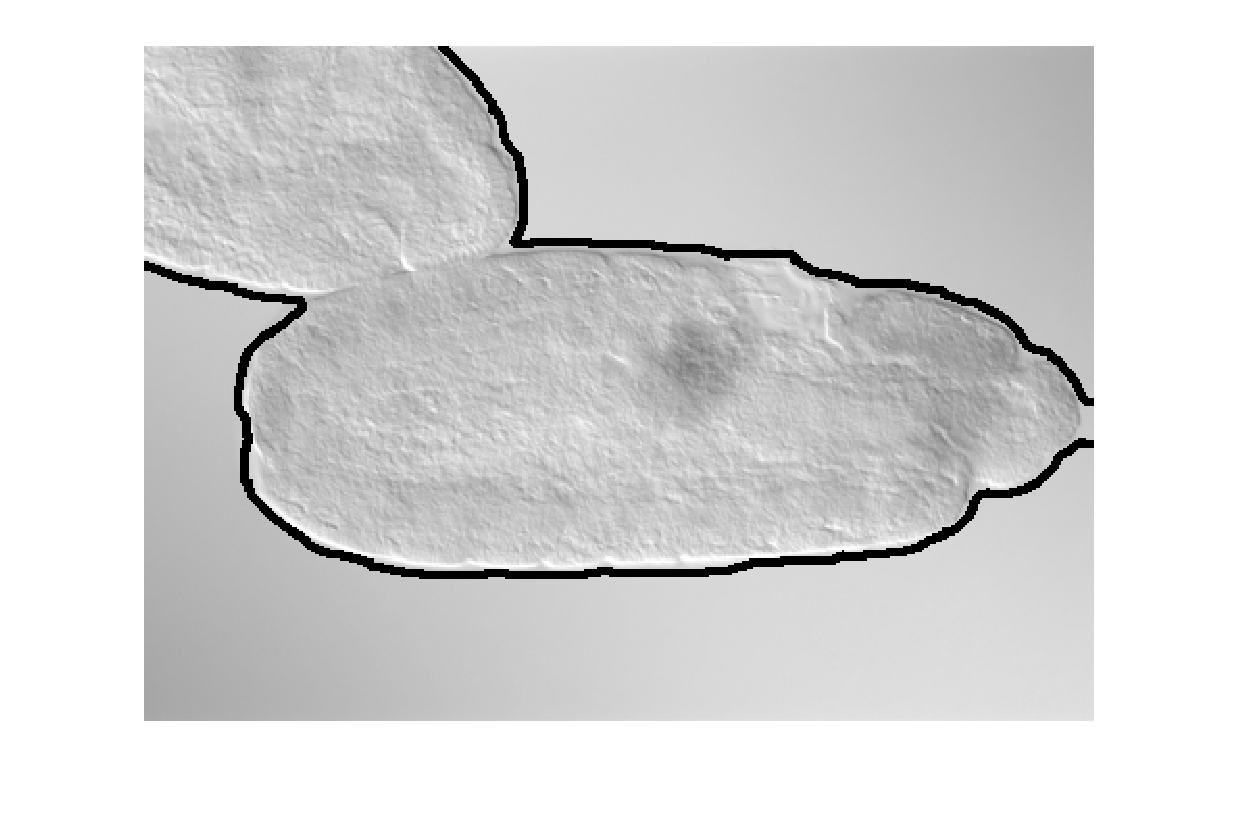
\includegraphics[width=150mm]{MRFtouching2.pdf}
  }
  \subfigure{
  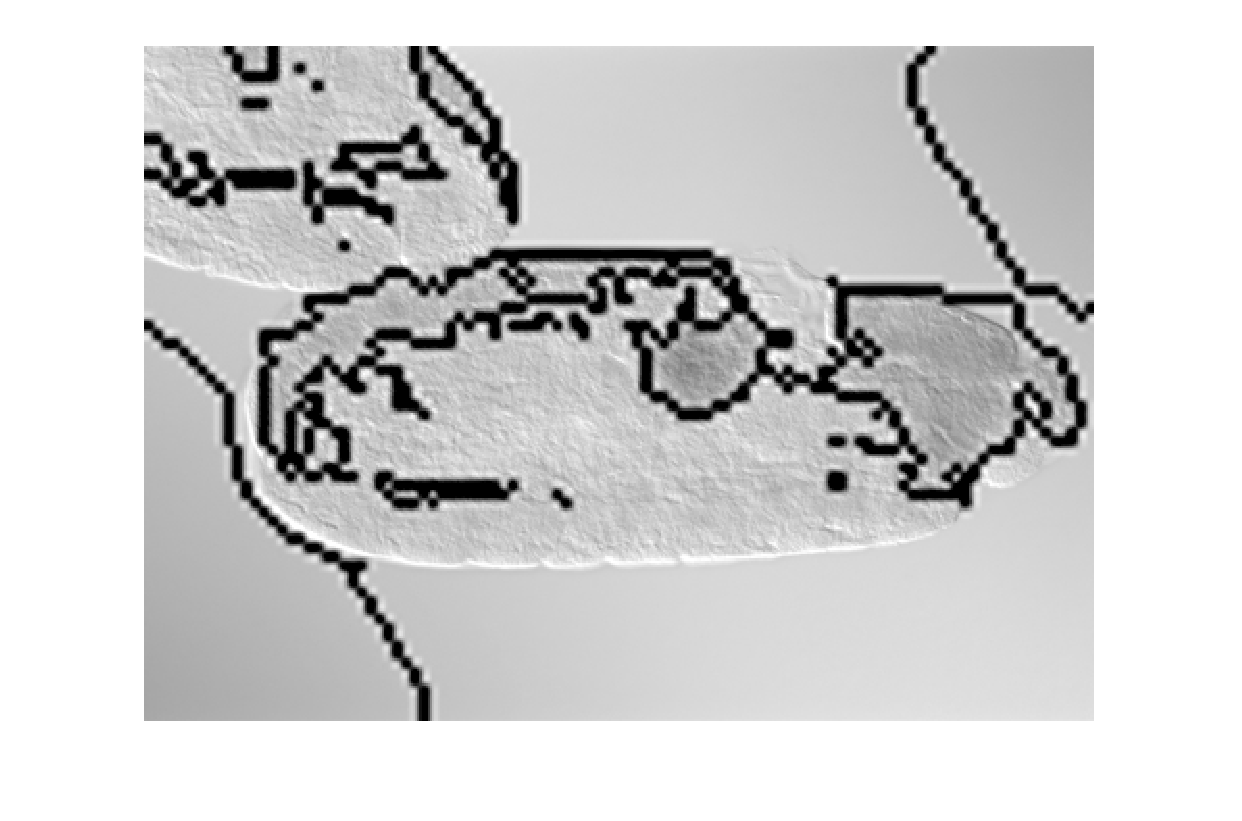
\includegraphics[width=150mm]{CVtouching2.pdf}
 }  
\caption{Left: MRF on superpixels. Right: Level set segmentation}
\label{Individual results}
 \end{figure}


%Segmentation Result running MRF combined with level set 
\begin{figure}[t]
  \centering
\subfigure{
  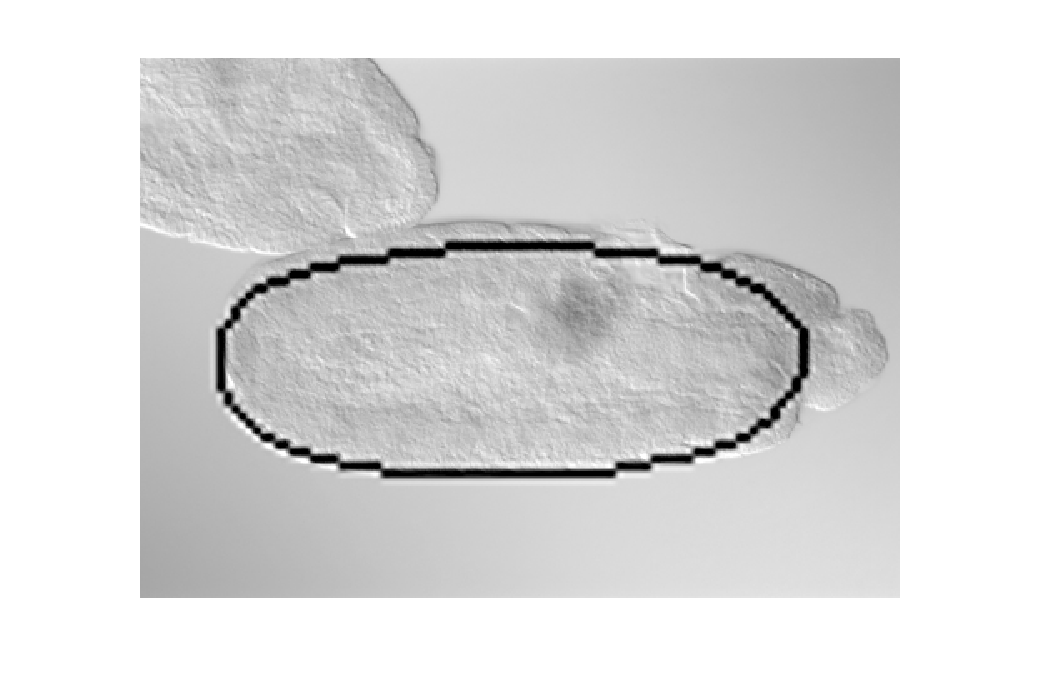
\includegraphics[width=150mm]{MRFCVtouching2.pdf}
 }  
  \subfigure{
    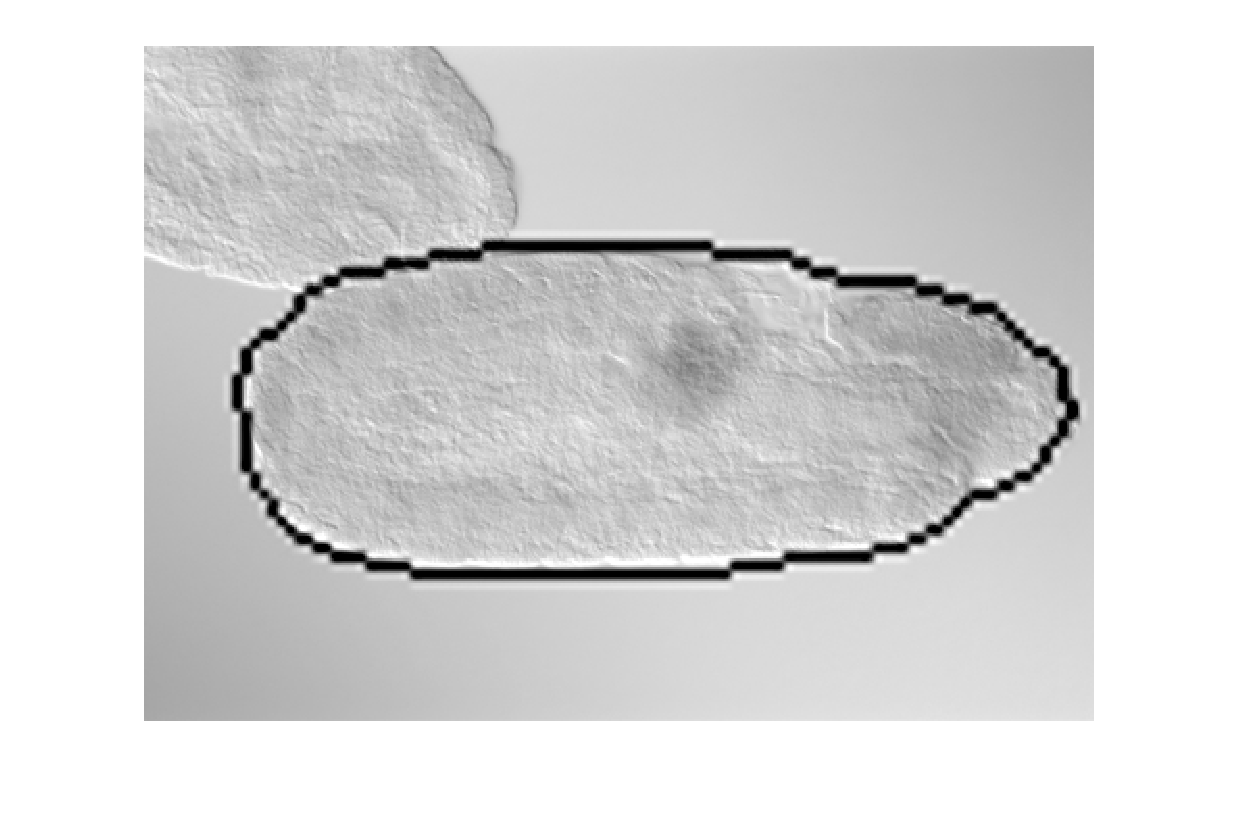
\includegraphics[width=150mm]{hybridPriorTouching2.pdf}
  }
  
\caption{Left: Level set segmentation and prior.  Right: MRF with level set segmentation}
\label{Individual results}
 \end{figure}


\end{examplelti}
% ===================================================================================================================


\begin{blocklti}{Future work}
\begin{itemize}
\item Multilabel extension
\item Application on the real problem: Segmentation of the gut, mouth etc.
\item Finding better features for MRF to speed up algorithm 
\end{itemize}

\end{blocklti}

\end{column2lti}

\end{columns}
\end{frame}


%%%%%%%%%%%%%%%%%%%%%%%%%%%%%%%%%%%%%%%%%%%%%%%%%%%%%%%%%%%%%%%%%%
\bibliographystyle{IEEEtran}
\bibliography{IEEEabrv,../publications,../pub_Pohl,../pub_Books}
%%%%%%%%%%%%%%%%%%%%%%%%%%%%%%%%%%%%%%%%%%%%%%%%%%%%%%%%%%%%%%%%%%

\end{document}
